\chapter{Code Specialization for Finite Element Integration}
\label{ch:coffee}

\section{Recapitulation and Objectives}
In Chapter~\ref{ch:optimality}, we have developed a method to minimize the operation count of finite element operators, or ``assembly kernels''. This chapter focuses on the same class of kernels, but tackles an orthogonal issue: low level optimization of generated code. We will abstract from the mathematical structure inherent in the expressions and concentrate on the aspects impacting the computational efficiency.

We know that an assembly kernel is characterized by the presence of an affine, often non-perfect loop nest, in which individual loops are rather small: their trip count rarely exceeds 30, and may be as low as 3 for low order methods. In the innermost loop, a problem-specific, compute intensive expression evaluates a two dimensional array, representing the result of local assembly in an element of the discretized domain. With such a kernel structure, we focus on aspects like register locality and SIMD vectorization.

We aim to maximize our impact on the platforms that are realistically used for finite element applications, so we target conventional CPU architectures rather than GPUs. The key limiting factor to the execution on GPUs is the stringent memory requirements. Only relatively small problems fit in a GPU memory, and support for distributed GPU execution in general purpose finite element frameworks is minimal. There has been some research on adapting local assembly to GPUs (mentioned later), although it differs from ours in several ways, including: (i) not relying on automated code generation from a domain-specific language (explained next), (ii) testing only very low order methods, (iii) not optimizing for cross-loop arithmetic intensity (the goal is rather effective multi-thread parallelization). In addition, our code transformations would drastically impact the GPU parallelization strategy, for example by increasing a thread's working set. For all these reasons, a study on extending the research to GPU architectures is beyond the scope of this work. In Section~\ref{sec:generality}, however, we provide some intuitions about this research direction.

Achieving high-performance on CPUs is non-trivial. The complexity of the mathematical expressions, which we know to be often characterized by a large number of operations on constants and small vectors, makes it hard to determine a single or specific sequence of transformations that is successfully applicable to all problems. Loop trip counts are typically small and can vary significantly, which further exacerbates the issue. The complexity of the memory access pattern also depends on the kernel, specifically on the function spaces employed by the method, ranging from unit-stride (e.g., \texttt{A[i]}, \texttt{A[i+1]}, \texttt{A[i+2]}, \texttt{A[i+3]}, ...) to random-stride (e.g., \texttt{A[i]}, \texttt{A[i+1]}, \texttt{A[i+2]}, \texttt{A[i+N]}, \texttt{A[i+N+1]}, ...). We will show that traditional vendor compilers, such as \emph{GNU's} and \emph{Intel's}, fail at maximizing the efficiency of the generated code because of such a particular structure. Polyhedral-model-based source-to-source compilers, for instance~\cite{pluto}, can apply aggressive loop optimizations, such as tiling, but these are not particularly helpful in our context since they mostly focus on cache locality. 

Like in Chapter~\ref{ch:optimality}, we focus on optimizing the performance of assembly kernels produced through automated code generation, so we seek transformations that are generally applicable and effective. In particular, we will study the following transformations:
\begin{description}
\item[Padding and data alignment] SIMD vectorization is more effective when the CPU registers are packed (unpacked) by means of aligned load (store) instructions. Data alignment is achieved through array padding, a conceptually simple yet powerful transformation that can result in dramatic reductions in execution time. We will see that the complexity of the transformation increases if non unite-stride memory accesses are present.
\item[Vector-register tiling] Blocking at the level of vector registers aims to improve data locality. This transformation exploits the peculiar memory access pattern inherent in finite element operators (i.e., inner products involving test and trial functions).  
\item[Expression splitting] Complex expressions are often characterized by high register pressure (i.e., the lack of available registers inducing the compiler to ``spill'' data from registers to cache). This happens, for example, when the number of arrays (e.g., basis functions, temporaries introduced by generalized code motion, temporaries produced by pre-evaluation) and constants is large compared to the number of available registers (typically 16 on state-of-the-art CPUs, 32 on future generations). This transformation exploits the associativity of addition to distribute, or ``split'', an expression into multiple sub-expressions; each sub-expression is then computed in a separate loop nest.
\item[Vector-expansion of invariant sub-expressions] In Chapter~\ref{ch:optimality} we have explained that some sub-expressions can be hoisted at the level of the integration loop. This transformation ``trades'' space for exposing a parallel dimension (the integration loop), thus promoting SIMD vectorization at the level of an outer loop.
\end{description}

To summarize, the contributions of this chapter are as follows:
\begin{itemize}
\item A number of low level transformations for optimizing the performance of assembly kernels.
\item Extensive experimentation using a set of real-world forms commonly arising in finite element methods.
\item A discussion concerning the generality of the transformations and their applicability to different domains.
\end{itemize}

\section{Low-level Optimization}
\label{sec:lowlevelopt}


\subsection{Padding and Data Alignment}
\label{sec:coffee-padding}
The absence of stencils renders the local element matrix computation easily auto-vectorizable by a general-purpose compiler. Nevertheless, auto-vectorization is not efficient if data are not aligned to cache-line boundaries and if the length of the innermost loop is not a multiple of the vector length $\mbox{\texttt{VL}}$, especially when the loops are small as in local assembly. 

Data alignment is enforced in two steps. Firstly, all arrays (but the element matrix, for reasons discussed shortly) are padded by rounding the innermost dimension to the nearest multiple of $\mbox{\texttt{VL}}$. For instance, assume the original size of a basis function array is 3$\times$3 and $\mbox{\texttt{VL}}=4$ (e.g. AVX processor, with 32-byte long vector registers and 8-byte double-precision floats). In this case, a padded version of the array will have size 3$\times$4. Secondly, their base address is enforced to multiples of $\mbox{\texttt{VL}}$ by means of special attributes. The compiler is explicitly told about data alignment using suitable pragmas; for example, in the case of the Intel compiler, the annotation \texttt{$\#$pragma vector aligned} is added before the loop (as shown in later figures) to inform that all of the memory accesses in the loop body will be properly aligned. This allows the compiler to issue aligned load and store instructions, which are notably faster than unaligned ones.

In our computational model, the element matrix is one of the kernel's input parameters, so it needs special handling when padding (the signature of the kernel must not be changed, otherwise the abstraction would be broken). We create a ``shadow'' copy of the element matrix, padded, aligned, and initialized to 0. The shadow element matrix is used in place of the original element matrix. Right before returning to the caller, a loop nest copies, discarding the padded region, the shadow matrix back into the input buffer.

Array padding also allows to safely round the loop trip count to the nearest multiple of $\mbox{\texttt{VL}}$. This avoids the introduction of a remainder (scalar) loop from the compiler, which would render vectorization less efficient. These extra iterations only write to the padded region of the element matrix, and therefore have no side effects on the final result.

Figure~\ref{code:helmholtz-licm-pad} illustrates the effect of padding and data alignment on top of generalized code motion applied to the weighted Laplace operator presented in Figure~\ref{code:weighted-laplace}.

\begin{algorithm}
\scriptsize\ttfamily
\SetAlgorithmName{LISTING}{}

\KwSty{void} weighted$\_$laplace(\KwSty{double} A[3][3], \KwSty{double} **coords, \KwSty{double} w[3]) $\lbrace$\\
~~\KwSty{$\#$define} ALIGN $\_\_$attribute$\_\_$((aligned(32))) \\
~~// K, det = Compute Jacobian (coords) \\
~~\\
~~// Quadrature weights \\
~~\KwSty{static const double} W[6] ALIGN = {0.5}; \\
~~\\
~~// Basis functions \\
~~\KwSty{static const double} B[6][4] ALIGN = $\lbrace\lbrace$...$\rbrace\rbrace$ ;\\
~~\KwSty{static const double} C[6][3] ALIGN = $\lbrace\lbrace$...$\rbrace\rbrace$ ;\\
~~\KwSty{static const double} D[6][4] ALIGN = $\lbrace\lbrace$...$\rbrace\rbrace$ ;\\
~~\\
~~// Padded buffer \\
~~\KwSty{double} $\_$A[3][4] ALIGN = $\lbrace\lbrace$0.0$\rbrace\rbrace$;\\
~~\\
~~\KwSty{for} (\KwSty{int} i = 0; i$<$6; i++) $\lbrace$ \\
~~~~\KwSty{double} f0  = 0.0;\\
~~~~\KwSty{for} (\KwSty{int} r  = 0; r < 3; ++r) $\lbrace$ \\
~~~~~~f0 += (w[r] * C[i][r]);\\
~~~~$\rbrace$ \\
~~~~\KwSty{double} T$\_$0[4] ALIGN;\\
~~~~\KwSty{double} T$\_$1[4] ALIGN;\\
~~~~\KwSty{for} (\KwSty{int} k = 0; k$<$4; r++) $\lbrace$ \\
~~~~~~T$\_$0[r] = ((K[1]*B[i][k])+(K[3]*D[i][k]));\\
~~~~~~T$\_$1[r] = ((K[0]*B[i][k])+(K[2]*D[i][k]));\\
~~~~$\rbrace$\\
~~~~\KwSty{for} (\KwSty{int} j = 0; j$<$3; j++) $\lbrace$\\
~~~~~~\KwSty{$\#$pragma vector aligned}\\
~~~~~~\KwSty{for} (\KwSty{int} k = 0; k$<$4; k++) $\lbrace$\\
~~~~~~~~$\_$A[j][k] += (T$\_$0[k]*T$\_$0[j] + T$\_$1[k]*T$\_$1[j])*det*W[i]*f0);\\
~~~~~~$\rbrace$\\
~~~~$\rbrace$\\
~~$\rbrace$\\
~~\KwSty{for} (\KwSty{int} j = 0; j$<$3; j++) $\lbrace$\\
~~~~\KwSty{for} (\KwSty{int} k = 0; k$<$3; k++) $\lbrace$\\
~~~~~~A[j][k] = $\_$A[j][k];\\
~~~~$\rbrace$\\
~~$\rbrace$\\
$\rbrace$

\caption{The assembly kernel for the weighted Laplace operator in Figure~\ref{code:weighted-laplace} after application of padding and data alignment (on top of generalized code motion). An AVX architecture, which implies $\mbox{\texttt{VL}}=4$, is assumed.}
\label{code:helmholtz-licm-pad}
\end{algorithm}

%\subsubsection{Example}
%Consider again the code in Figure~\ref{fig:withzeros-skipped-code} and assume $\mbox{\texttt{VL}}=4$ double-precision floats (i.e. vector registers are 32 bytes longs). 
%
%The arrays in the loop nest \texttt{[j1,k1]} can be padded and the right bound of loop \texttt{k1} can be safely increased to 8: eventually, values computed in the region \texttt{M[0:3][6:8]} will be discarded. Then, by explicitly aligning arrays using suitable qualifiers (e.g. \texttt{$\#\_\_$attribute$\_\_$((aligned(32)))} for the Intel compiler), effective SIMD auto-vectorization can be obtained for this loop nest. 
%
%There are some complications in the case of loops \texttt{[j0,k0]}. Here, increasing the innermost loop bound to 4 is still safe assuming that both \texttt{T1} and \texttt{A} are padded, but it has no effect: the starting addresses of the load instructions would be \texttt{$\&$T1[3]} and \texttt{$\&$A[i][3]}, which are clearly not aligned. Changing the starting address of \texttt{A} and \texttt{T1} is, in general, not an option, because these arrays could be accesses also in other loop nests, as happens with \texttt{A} in this example. One solution, instead, is to start iterating from the closest index that would ensure data alignment; in this case, $k0=0$. However, this would imply losing the effect of the zero-avoidance transformation (partially in general, totally for this loop nest). Another possibility is to attain to non-aligned accesses. Which of the two strategies is better cannot be established a-priori. An autotuning system, as described in Section~\ref{sec:coffee-autotune}, will help answering this question.
%
%Finally, note that whenever increasing a loop bound cause accessing non-zero entries in the local element matrix \texttt{M}, there is no way of recovering data alignment.

\subsection{Expression Splitting}
\label{sec:coffee-split}

In complex kernels, like Burgers in Listing~\ref{code:burgers}, and on certain architectures, achieving effective register allocation can be challenging. If the number of variables independent of the innermost-loop dimension is close to or greater than the number of available CPU registers, poor register reuse is likely. This usually happens when the number of basis function arrays, temporaries introduced by generalized loop-invariant code motion, and problem constants is large. For example, applying loop-invariant code motion to Burgers on a 3D mesh requires 24 temporaries for the \texttt{ijk} loop order. This can make hoisting of the invariant loads out of the \texttt{k} loop inefficient on architectures with a relatively low number of registers. One potential solution to this problem consists of suitably ``splitting'' the computation of the element matrix $A$ into multiple sub-expressions; an example, for the Burgers problem, is given in Listing~\ref{code:burgers-split}. The transformation can be regarded as a special case of classic loop fission, in which associativity of the sum is exploited to distribute the expression across multiple loops. To the best of our knowledge, expression splitting is not supported by available compilers.

\begin{algorithm}
\scriptsize\ttfamily
\SetAlgorithmName{LISTING}{}

\KwSty{void} helmholtz(\KwSty{double} A[3][4], \KwSty{double} **coords) $\lbrace$\\
~~~~// Same code as in Listing~\ref{code:helmholtz-licm} up to the j loop\\
~~~~\KwSty{for} (\KwSty{int} j = 0; j$<$3; j++) \\
~~~~~~\KwSty{$\#$pragma vector aligned}\\
~~~~~~\KwSty{for} (\KwSty{int} k = 0; k$<$4; k++) \\
~~~~~~~~A[j][k] += (Y[i][k]*Y[i][j]+LI$\_$0[k]*LI$\_$0[j])*det*W3[i];\\
~~~~\KwSty{for} (\KwSty{int} j = 0; j$<$3; j++) \\
~~~~~~\KwSty{$\#$pragma vector aligned}\\
~~~~~~\KwSty{for} (\KwSty{int} k = 0; k$<$4; k++) \\
~~~~~~~~A[j][k] += LI$\_$1[k]*LI$\_$1[j]*det*W3[i];\\
$\rbrace$
\caption{Local assembly code generated by Firedrake for the Helmholtz
  problem in which \emph{split} has been applied on top of the
  optimizations shown in Listing~\ref{code:helmholtz-licm}. In this
  example, the split factor is 2.}
\label{code:helmholtz-split}
\end{algorithm}

Splitting an expression (henceforth \emph{split}) has, however, several drawbacks. Firstly, it increases the number of accesses to $A$ proportionally to the ``split factor'', which is the number of sub-expressions produced. Also, depending on how the split is executed and the way expression rewriting is performed, it can lead to redundant computation. For example, the number of times the product $det*W3[i]$ is performed is proportional to the number of sub-expressions, as shown in the code snippet. Further, it increases loop overhead, for example through additional branch instructions. Finally, it might affect register locality: for instance, the same array could be accessed in different sub-expressions, requiring a proportional number of loads be performed; this, again, depends on expression rewriting. Nevertheless, as shown in Section~\ref{sec:coffee-perfeval-single}, the performance gain from improved register reuse along inner dimensions can be important, especially if the selection of the split factor uses heuristics to minimize the aforementioned issues.

\subsection{Model-driven Vector-register Tiling}
\label{sec:coffee-opvect}

\begin{algorithm}
\tiny\ttfamily
\SetAlgorithmName{LISTING}{}

\begin{multicols}{2}
\KwSty{void} helmholtz(\KwSty{double} A[4][4], \KwSty{double} **coords) $\lbrace$\\
~~// K, det = Compute Jacobian (coords) \\
~~// Declaration of basis function matrices \\
~~\\
~~\KwSty{for} (\KwSty{int} i = 0; i$<$3; i++) $\lbrace$ \\
~~~~// Do generalized loop-invariant code motion \\
~~~~\KwSty{for} (\KwSty{int} j = 0; j$<$4; j+=4) \\
~~~~~~\KwSty{for} (\KwSty{int} k = 0; k$<$4; k+=4) $\lbrace$\\
~~~~~~~~// \emph{load} and \emph{set} intrinsics \\
~~~~~~~~// Compute A[0,0], A[1,1], A[2,2], A[3,3] \\
~~~~~~~~// One \emph{permute\_pd} intrinsic per \texttt{k}-loop \emph{load}\\
~~~~~~~~// Compute A[0,1], A[1,0], A[2,3], A[3,2] \\
~~~~~~~~// One \emph{permute2f128\_pd} intrinsic per \texttt{k}-loop \emph{load}\\
~~~~~~~~// ...\\
~~~~~~$\rbrace$\\
~~~~// Remainder loop (from $j=4$ to $j=6$)\\
~~$\rbrace$\\
~~// Restore the storage layout:\\
~~\KwSty{for} (\KwSty{int} j = 0; j$<$4; j+=4) $\lbrace$\\
~~~~\KwSty{$\_\_$m256d} r0, r1, r2, r3, r4, r5, r6, r7;\\
~~~~\KwSty{for} (\KwSty{int} k = 0; k$<$4; k+=4) $\lbrace$\\
~~~~~~r0 = $\_$mm256$\_$load$\_$pd ($\&$A[j+0][k]);\\
~~~~~~// Load A[j+1][k], A[j+2][k], A[j+3][k]\\
~~~~~~r4 = $\_$mm256$\_$unpackhi$\_$pd (r1, r0);\\
~~~~~~r5 = $\_$mm256$\_$unpacklo$\_$pd (r0, r1);\\
~~~~~~r6 = $\_$mm256$\_$unpackhi$\_$pd (r2, r3);\\
~~~~~~r7 = $\_$mm256$\_$unpacklo$\_$pd (r3, r2);\\
~~~~~~r0 = $\_$mm256$\_$permute2f128$\_$pd (r5, r7, 32);\\
~~~~~~r1 = $\_$mm256$\_$permute2f128$\_$pd (r4, r6, 32);\\
~~~~~~r2 = $\_$mm256$\_$permute2f128$\_$pd (r7, r5, 49);\\
~~~~~~r3 = $\_$mm256$\_$permute2f128$\_$pd (r6, r4, 49);\\
~~~~~~$\_$mm256$\_$store$\_$pd ($\&$A[j+0][k], r0);\\
~~~~~~// Store A[j+1][k], A[j+2][k], A[j+3][k]\\
~~~~$\rbrace$\\
~~$\rbrace$\\
$\rbrace$
\end{multicols}
\caption{Local assembly code generated by Firedrake for the Helmholtz
  problem after application of \emph{op-vect} on top of the
  optimizations shown in Listing~\ref{code:helmholtz-licm}. In this
  example, the unroll-and-jam factor is 1.}
\label{code:helmholtz-opvect}
\end{algorithm}

One notable problem of assembly kernels concerns register allocation and register locality. The critical situation occurs when loop trip counts and the variables accessed are such that the vector-register pressure is high. Since the kernel's working set fits the L1 cache, it is particularly important to optimize register management. Standard optimizations, such as loop interchange, unroll, and unroll-and-jam, can be employed to deal with this problem. Tiling at the level of vector registers represents another opportunity. Based on the observation that the evaluation of the element matrix can be reduced to a summation of outer products along the \texttt{j} and \texttt{k} dimensions, a model-driven vector-register tiling strategy can be implemented. If we consider the codes in the various listings and we focus on the body of the test and trial functions loops (\texttt{j} and \texttt{k}), the computation of the element matrix is abstractly expressible as
\begin{equation}
\scriptsize
\label{outer-product}
A_{jk} = \sum_{\substack{
  x \in B' \subseteq B \\
  y \in B'' \subseteq B}}
x_j\cdot y_k ~~~~~~ j,k = 0,...,2
\end{equation}
where $B$ is the set of all basis functions (or temporary variables, e.g., \texttt{LI$\_$0}) accessed in the kernel, whereas $B'$ and $B''$ are generic problem-dependent subsets. Regardless of the specific input problem, by abstracting from the presence of all variables independent of both \texttt{j} and \texttt{k}, the element matrix computation is always reducible to this form. Figure~\ref{fig:vect-by-vect} illustrates how we can evaluate 16 entries ($j,k=0,...,3$) of the element matrix using just 2 vector registers, which represent a 4$\times$4 tile, assuming $\vert B' \vert = \vert B'' \vert = 1$. Values in a register are shuffled each time a product is performed. Standard compiler auto-vectorization for both GNU and Intel compilers, instead, executes 4 broadcast operations (i.e., ``splat'' of a value over all of the register locations) along the outer dimension to perform the calculation. In addition to incurring a larger number of cache accesses, it needs to keep between $f=1$ and $f=3$ extra registers to perform the same 16 evaluations when unroll-and-jam is used, with $f$ being the unroll-and-jam factor.

%More importantly, we avoid using $\mbox{\texttt{VL}}$-1 registers per each
%outer-loop-dependent variable (i.e., all $x$ terms in
%Equation~\ref{outer-product}), with $\mbox{\texttt{VL}}$ being the vector
%length. This is a considerable gain, which allows us to slice the
%iteration space into bigger tiles, implemented directly by vector
%registers.

\begin{figure}
\centerline{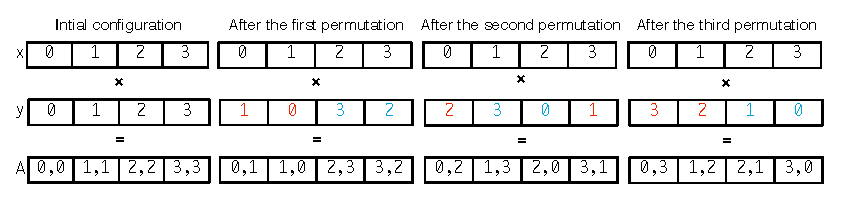
\includegraphics[scale=0.6]{coffee/pictures/vect-by-vect-inline.pdf}}
\caption{Outer-product vectorization by permuting values in a vector register.}
\label{fig:vect-by-vect}
\end{figure}

The storage layout of $A$, however, is incorrect after the application of this outer-product-based vectorization (\emph{op-vect}, in the following). It can be efficiently restored with a sequence of vector shuffles following the pattern highlighted in Figure~\ref{fig:restore-layout}, executed once outside of the \texttt{ijk} loop nest. The pseudo-code for the Burgers local assembly kernel when using \emph{op-vect} is shown in Listing~\ref{code:burgers-opvect}.

\begin{figure}
\centerline{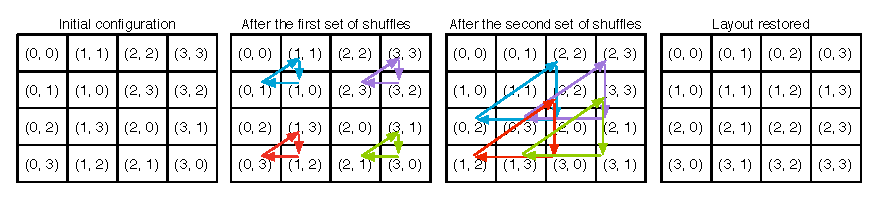
\includegraphics[scale=0.6]{coffee/pictures/vect-restore-inline.pdf}}
\caption{Restoring the storage layout after \emph{op-vect}. The figure shows how 4$\times$4 elements in the top-left block of the element matrix $A$ can be moved to their correct positions. Each rotation, represented by a group of three same-colored arrows, is implemented by a single shuffle intrinsic.}
\label{fig:restore-layout}
\end{figure}

\subsection{Vector-expansion of Invariant Sub-expressions}
\label{sec:coffee-precompute}
...
%\begin{figure}
%\centering
%\footnotesize
%\lstinputlisting{coffee/listings/vectexpanded.code}
%\caption{Local assembly code for the Burgers example after precomputation and scalar-expansion of loop-invariant terms.}
%\label{code:scalarexp-code}
%\end{figure}
%
%We note that integration-dependent expressions are inherently executed as scalar code. For example, the \texttt{f0*a} and \texttt{f1*b} products in Figure~\ref{code:factorized-code} depend on the loop along quadrature points; these operations are performed in a non-vectorized way at every \texttt{i} iteration. This is not a big issue in our running example, in which the scalar computation represents a small fraction of the total, but it becomes a concrete problem in complicated forms, like those at the heart of hyperelasticity (which will be part of our performance evaluation). In such forms, the amount of computation independent of both test and trial functions loops is so large that it has a significant impact on the run-time, despite being executed only $O(I)$ times (with $I$ number of quadrature points). We have therefore implemented an algorithm to move and scalar-expand integration-dependent expressions, which leads to codes as in Figure~\ref{code:scalarexp-code}.




\section{Implementation in COFFEE}
\label{sec:coffee-implementation}
\subsection{Outline and Integration with Firedrake}

\begin{figure}
\begin{center}
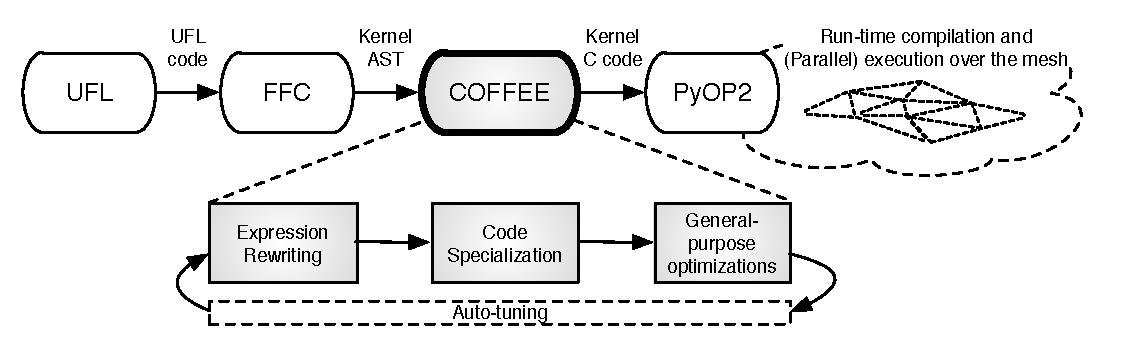
\includegraphics[scale=0.70]{coffee/pictures/coffee-pipeline.pdf}
\caption{High-level view of Firedrake. COFFEE is at the core, receiving ASTs from a modified version of the FEniCS Form Compiler and producing optimized C code kernels.}
\label{fig:coffee-pipeline}
\end{center}
\end{figure}

Our research resulted in the implementation of COFFEE\footnote{COFFEE stands for COmpiler For FinitE Element local assembly.}, a mature, platform-independent compiler capable of optimizing any local assembly code generated through Firedrake or FEniCS. COFFEE has been fully integrated with Firedrake, so it can optimize any equation expressible with this framework. The code, which comprises more than 5000 lines, is available at~\citep{coffee-code}.

Firedrake users employ the Unified Form Language to express problems in a notation resembling mathematical equations. At run-time, the high-level specification is translated by a modified version of its form compiler, the FEniCS Form Compiler (FFC)~\cite{FFC-Compiler}, into an abstract syntax tree (AST) representation of one or more finite element assembly kernels. ASTs are then passed to COFFEE to apply the transformations described in the previous sections. The output of COFFEE, C code, is eventually provided to PyOP2~\citep{pyop2isc}, where just-in-time compilation and execution over the discretized domain take place. The flow and the compiler structure are outlined in Figure~\ref{fig:coffee-pipeline}. 

The compiler applies an ordered sequence of optimization steps to the ASTs received from FFC. Expression rewriting is performed first, due to the introduction of temporary arrays and the need to create multiple loop nest starting from the original one (this may happen when computation over zero-valued blocks is avoided). Then, code specialization takes place. Finally, loop interchange and loop unroll are applied. COFFEE has an auto-tuning system, described in Section~\ref{sec:coffee-autotune}, to individuate the most suitable optimization strategy (i.e. to select which transformations to apply) for a certain equation. The implementation of all code transformations is centered on analysis and manipulation of the kernel AST. Any possible corner cases are handled: for example, if outer-product vectorization is to be applied but the size of the iteration space is not a multiple of the vector length, then a remainder loop, amenable to auto-vectorization, is inserted (as shown in Figure~\ref{code:burgers-opvect}).

Users can either enable individual transformations by switching specific flags or leave the auto-tuning system, described in Section~\ref{sec:coffee-autotune}, in charge of determining the best optimization strategy (i.e. selecting and composing transformations).

\subsection{Modifying the FEniCS Form Compiler}
COFFEE expects as input either a string of C code or an AST. In the former case, a parser could be used to obtain an AST representation, which is required by the algorithms implementing the various code transformations. Therefore, FFC's output, which is a C-code implementation of a local assembly kernel, could be used straightforwardly as input to COFFEE. However, we note that this would also be conceptually pointless: FFC would generate C code from its intermediate representation that eventually COFFEE would have to re-parse to obtain an AST. A much cleaner solution, adopted and explained next, consists of modifying FFC to directly generate an AST. 

\subsubsection{Generation of Abstract Syntax Trees}
The construction of the FFC's intermediate representation from UFL code is refined as follows:
\begin{itemize}
\item The mathematical expression that evaluates the element matrix is represented by a tree data structure. A limitation of the original FFC was that nodes in such expression tree, which correspond to symbols or arithmetic operations, are not bound to the enclosing loops. For instance, consider the symbol \texttt{A[i][j]}: the FFC's expression tree has a node for this symbol, but visiting it there is no clean way of separating the variable name \texttt{A} from the loop indices \texttt{i} and \texttt{j}. Therefore, we have enriched symbol nodes with additional fields to capture these information. 
\item Basis functions in the FFC's intermediate representation are characterized by a new field telling whether they originated from a vector-valued or a scalar-valued element. In the former case, the array rappresenting the tabulation of a basis function at the various quadrature points is block-sparse. This information is recorded and, as explained next, attached to the kernel's AST to enable COFFEE applying symbolic execution to avoid iteration over zero-valued blocks, as elaborated in Section~\ref{sec:coffee-avoidzeros}.
\end{itemize}
In the modified FFC, the intermediate representation is intercepted prior to the code generation stage and forwarded to a new module that builds ASTs. To this purpose, COFFEE exposes its hierarchy of AST nodes, whose design strictly adhere to standard object-oriented programming rules (e.g. by making extensive use of overloading). An example of such an AST representation for a simple C statement is provided in Figure~\ref{fig:coffee-ast-vs-c}.

\begin{figure}
\begin{center}
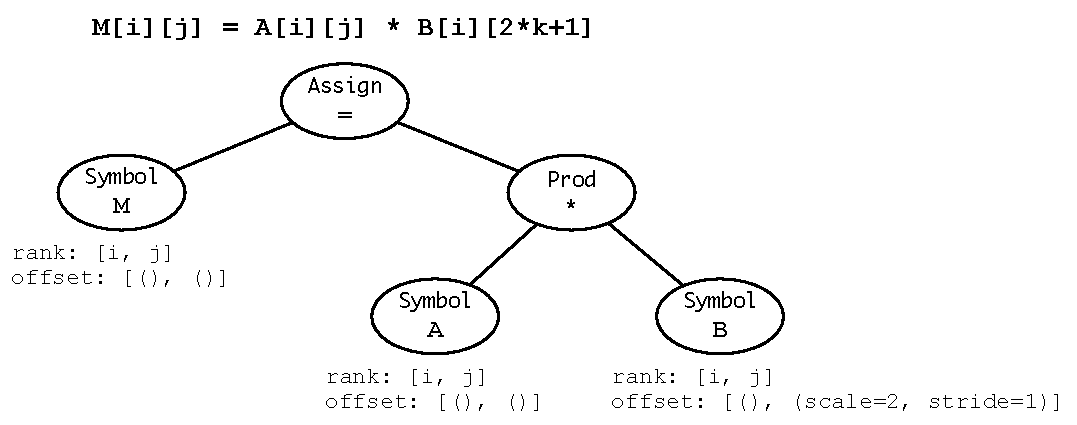
\includegraphics[scale=0.50]{coffee/pictures/coffee-ast.pdf}
\caption{AST representation of a C assignment in COFFEE.}
\label{fig:coffee-ast-vs-c}
\end{center}
\end{figure}

The enriched intermediate representation allows to create proper AST's Symbol nodes. A Symbol, as shown in the figure, has a name (the variable name), an array of indices, and an array of offsets. These information are fundamental for the implementation of expression rewriting and code specialization. Further, special AST's Declaration objects can be used to track the sparsity pattern in basis function arrays. 

\subsection{On the Compiler Implementation}

\begin{figure}
\begin{center}
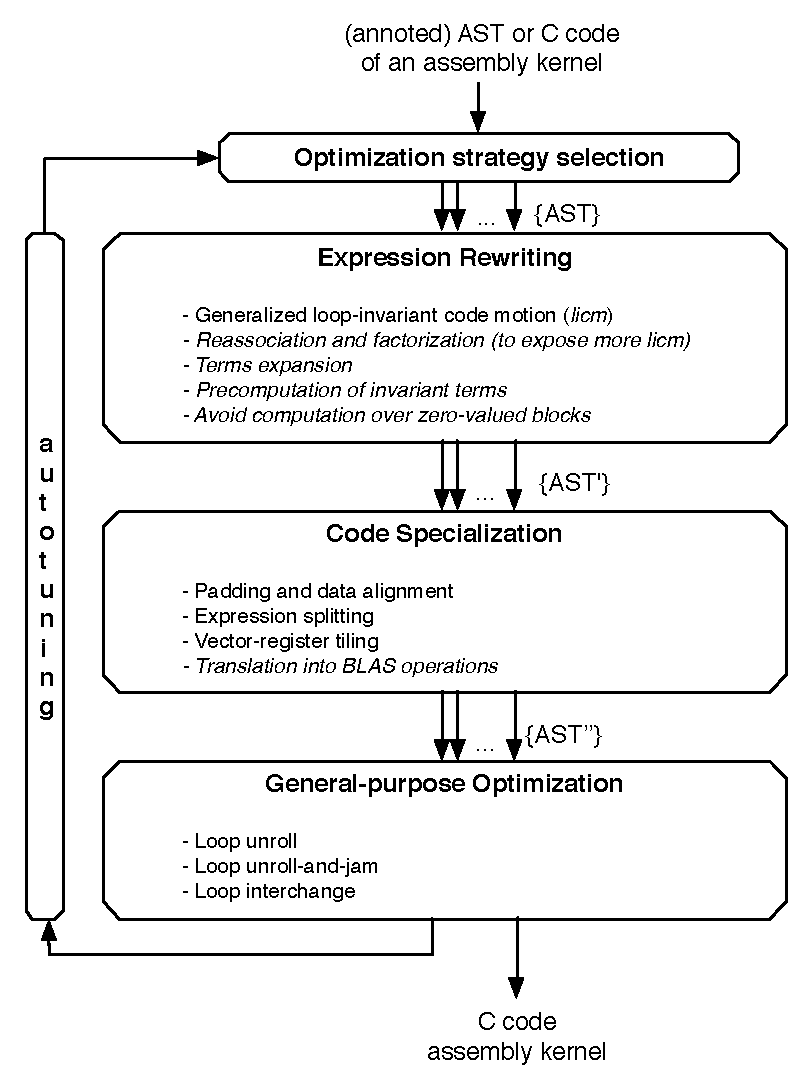
\includegraphics[scale=0.70]{coffee/pictures/coffee-scheme.pdf}
\caption{Structure of COFFEE.}
\label{fig:coffee-compiler-structure}
\end{center}
\end{figure}

Figure~\ref{fig:coffee-compiler-structure} outlines the various modules composing COFFEE. Expression rewriting, code specialization, and general-purpose transformations are applied by manipulating the AST representing the local assembly kernel. Providing the steps of all algorithms performing the various transformations would just be tedious and marginally helpful for the reader; essentially, implementing a transformation always reduces to write a routine that visits and manipulates a tree data structure (the AST) according to the semantics described in Sections~\ref{sec:coffee-expr-rewrite} and~\ref{sec:coffee-code-spec}. In this section, we rather focus on aspects of the compiler implementation that involve the orchestration of the different transformations, including a description of the data structures employed to track both the restructuring of the assembly expressions and data dependencies. 

\subsubsection{Code Hoisting}
Hoisting is the operation of moving code, for instance a statement or the evaluation of an expression, from an inner to an outer loop in a nest. This operation is performed in several occasions when rewriting an expression: generalized loop-invariant code motion, expansion of sub-expressions, and precomputation of terms all require code hoisting, as illustrated in Figures~\ref{code:invariant-code} and~\ref{code:expanded-code}. In order to perform code hoisting, in particular, several aspects must be known:
\begin{enumerate}
\item ``what'' to hoist
\item ``where'' to hoist (possibly, outside of the loop nest)
\item if scalar-expansion should be introduced
\end{enumerate}
Answers to these three points obviously depend on the specific transformation, although parts of the implementation are shared. COFFEE tracks hoisted code by means of a dictionary that binds variable names (guaranteed to be unique) to a set of information. In particular, for a variable \texttt{v}, the dictionary provides:
\begin{itemize}
\item a reference to the AST node corresponding to the expression \texttt{e} hosted by \texttt{v};
\item a reference to the loop in which \texttt{v} is assigned \texttt{e};
\item a reference to the AST node corresponding to the declaration of \texttt{v}.
\end{itemize}
As expressions are hoisted, the dictionary is populated and/or updated with new information. For example, when applying generalized loop-invariant code motion, a new entry is created, unless the sub-expression being lifted has already been pre-computed elsewhere. On the other hand, when sub-expressions are expanded, either a new entry is created or an old entry is updated, as explained in Section~\ref{sec:coffee-expansion}. 

The dictionary is also queried at code specialization time for padding, data alignment and generation of BLAS calls. Therefore, different algorithms in COFFEE access the same data structure, which allows avoiding both duplicated code and an additional overhead due to revisiting the same portion of AST in distinct transformations.

\subsubsection{Benefits of Tracking Data Dependencies}
COFFEE implements ``smart'' code hoisting: everytime a sub-expression or a term are lifted, for example from the mathematical expression evaluating the local element matrix to an outer level in the loop nest, three optimizations are potentially applied. Consider a hoistable expression \texttt{e} assuming different values in the iteration space \texttt{I}:
\begin{itemize}
\item \textbf{Minimize redundant computation.} If an equivalent sub-expression \texttt{e'} has already been hoisted along the iteration space \texttt{I}, then COFFEE replaces \texttt{e} with a reference to the symbol hosting the value of \texttt{e'}. This avoids both redundant computation and the introduction of additional temporary variables;
\item \textbf{Loop fusion.} If scalar-expansion is introduced (we recall this is useful to achieve SIMD auto-vectorization; see Sections~\ref{sec:coffee-licm} and~\ref{sec:coffee-precompute}), then the hoisted code must be placed in an outer loop \texttt{r}, \texttt{r $\in$ I}. This was the purpose of the second \texttt{r} loop in Figure~\ref{code:invariant-code}; note that this loop includes scalar-expanded sub-expressions that, in the non-transformed code, iterated along logically different spaces (loops \texttt{j} and \texttt{k}, corresponding to test and trial functions). In this example, it was possible to use a single \texttt{r} loop because we assumed that test and trial function spaces were the same, leading to identical loop bounds; in general, however, this is not true. Another assumption of the example was that the space of the equation's coefficients (variables \texttt{f0, f1} in the figure) coincided with that of test and trial functions. This would allow fusing the two \texttt{r} loops, which is exactly what COFFEE does, although not displayed by the figure. Fusing loops, which increases data locality and reduces loop overhead, is possible in some circumnstances, in particular when there are no data dependencies among hoisted expressions and the spaces of test, trial, and coefficent functions are identical. As explained next, COFFEE reasons about data dependencies and iteration spaces to determine the safeness of loop fusion.
\item \textbf{Reduce extra memory.} When expanding an expression, terms hoisting is possible to relieve register pressure. This poses the challenge described in Section~\ref{sec:coffee-expansion} and intuitively summarized in Figure~\ref{code:expanded-code}; that is, understanding whether it is possible to absorb the hoistable term in an available temporary value or a new temporary is needed. Obviously, the less is the number of temporaries introduced, the smaller is the size of the working set, which may result in better performance.
\end{itemize}
To implement these optimizations, it is necessary to track the evolution of data dependencies as the assembly expression is rewritten. For this purpose, COFFEE uses a dependency graph, which is a standard approach used by general-purpose compilers relying on abstract syntax trees (in addition to other data structures) as intermediate representation. The dependency graph has as many nodes as the number of variables in the loop nest characterizing the assembly expression. A direct edge from a node \texttt{A} to a node \texttt{B} indicates that the value of symbol \texttt{B} depends on that of \texttt{A}. 

The implementation of the depedency graph data structure and of the various algorithms using it is made simple by the fact that COFFEE ensures \textit{static single assignment} form. This property, typically adopted by intermediate representations in compilers, requires that variables are assigned exactly once, and that each variable is defined in advance. 


\section{Experiments}
\label{sec:coffee-perfeval}

\subsection{Experimental Setup}
\label{sec:coffee-perfeval-setup}
Experiments were run on a single core of an Intel architecture, a Sandy Bridge I7-2600 CPU running at 3.4GHz, with 32KB of L1 cache and 256KB of L2 cache). The \texttt{icc 14.1}  compiler was used. On the Sandy Bridge, the compilation flags used were \texttt{-O2} and \texttt{-xAVX} for auto-vectorization. Other optimization levels performed, in general, slightly worse.

Three studies are presented. Firstly, in Section~\ref{sec:coffee-perfeval-single}, the impact of individual code transformations is analyzed in three real-world, representative equations. We believe it is important to clarify \textit{in which contexts} and \textit{why} such optimizations can provide speed ups. 

...

\subsection{Rationale of the Study}
\label{sec:coffee-individual-rationale}
We evaluate some critical code transformations in three real-world problems based on the following PDEs: (i) Helmholtz, (ii) Diffusion, and (iii) Burgers. The evaluation concerns:
\begin{itemize}
\item Generalized loop-invariant code motion (Section~\ref{sec:coffee-licm})
\item Padding and data alignment (Section~\ref{sec:coffee-padding})
\item Expression splitting (Section~\ref{sec:coffee-split})
\item Vector-register tiling (Section~\ref{sec:coffee-opvect})
\end{itemize}
\textit{The goal of this section is to demonstrate the effectiveness of individual transformations and to explain under what circumnstances performance improvements are obtainable}. It is important to understand \textit{for what reasons} gains in run-time are achieved with these critical optimizations; some transformations are excluded from this study for reasons of time and readability of the section, but analogous considerations and observations would apply. 
%However, in Section~\ref{sec:coffee-perfeval-allforms}, we will show that an aggressive optimization strategy based on extensive expression rewriting, code specialization, and exploitation of COFFEE's auto-tuning system can outperform the cumulative impact of the transformations analyzed in the present section.

The three chosen equations are \emph{real-life kernels} and comprise the core differential operators in some of the most frequently encountered finite element problems in scientific computing. This is of crucial importance because distinct problems, possibly arising in completely different fields, may employ (subsets of) the same differential operators of our benchmarks, which implies similarities and redundant patterns in the generated code. Consequently, the proposed code transformations have a domain of applicability that goes far beyond that of the three analyzed equations.

The Helmholtz and Diffusion kernels are archetypal second order elliptic operators. They are complete and unsimplified examples of the operators used to model diffusion and viscosity in fluids, and for imposing pressure in compressible fluids. As such, they are both extensively used in climate and ocean modeling. Very similar operators, for which the same optimisations are expected to be equally effective, apply to elasticity problems, which are at the base of computational structural mechanics. The Burgers kernel is a typical example of a first order hyperbolic conservation law, which occurs in real applications whenever a quantity is transported by a fluid (the momentum itself, in our case). We chose this particular kernel since it applies to a vector-valued quantity, while the elliptic operators apply to scalar quantities; this impacts the generated code, as explained next. The operators we have selected are characteristic of both the second and first order operators that dominate fluids and solids simulations.
%and a wide variety on local assembly codes can be tested.

The benchmarks were written in UFL (code available at~\citep{ufl-code-individual}) and executed over real unstructured meshes through Firedrake. The Helmholtz code has already been shown in Listing~\ref{code:helmholtz}. The Diffusion equation uses the same differential operators as Helmholtz. In the Diffusion kernel code, the main differences with respect to Helmholtz are the absence of the $Y$ array and the presence of additional constants for computing the element matrix. Burgers is a non-linear problem employing differential operators different from those of Helmholtz and relying on vector-valued quantities, which has a major impact on the generated assembly code (see Listing~\ref{code:burgers}), where a larger number of basis function arrays ($X1$, $X2$, ...) and constants ($F0$, $F1$, ..., $K0$, $K1$,
...) are generated. 

These problems were studied varying both the shape of mesh elements and the polynomial order $q$ of the method, whereas the element family, Lagrange, is fixed. As might be expected, the larger the element shape and $q$, the larger the iteration space. Triangles, tetrahedra, and prisms were tested as element shape. For instance, in the case of Helmholtz with $q=1$, the size of the \texttt{j} and \texttt{k} loops for the three element shapes is, respectively, $3$, $4$, and $6$. Moving to bigger shapes has the effect of increasing the number of basis function arrays, since, intuitively, the behaviour of the equation has to be approximated also along a third axis. On the other hand, the polynomial order affects only the problem size (the three loops \texttt{i}, \texttt{j}, and \texttt{k}, and, as a consequence, the size of $X$ and $Y$ arrays). A range of polynomial orders from $q=1$ to $q=4$ were tested; higher polynomial orders are excluded from the study because of current Firedrake limitations. In all these cases, the size of the element matrix rarely exceeds 30$\times$30, with a peak of 105$\times$105 in Burgers with prisms and $q=4$.

\begin{figure}[t]
\centerline{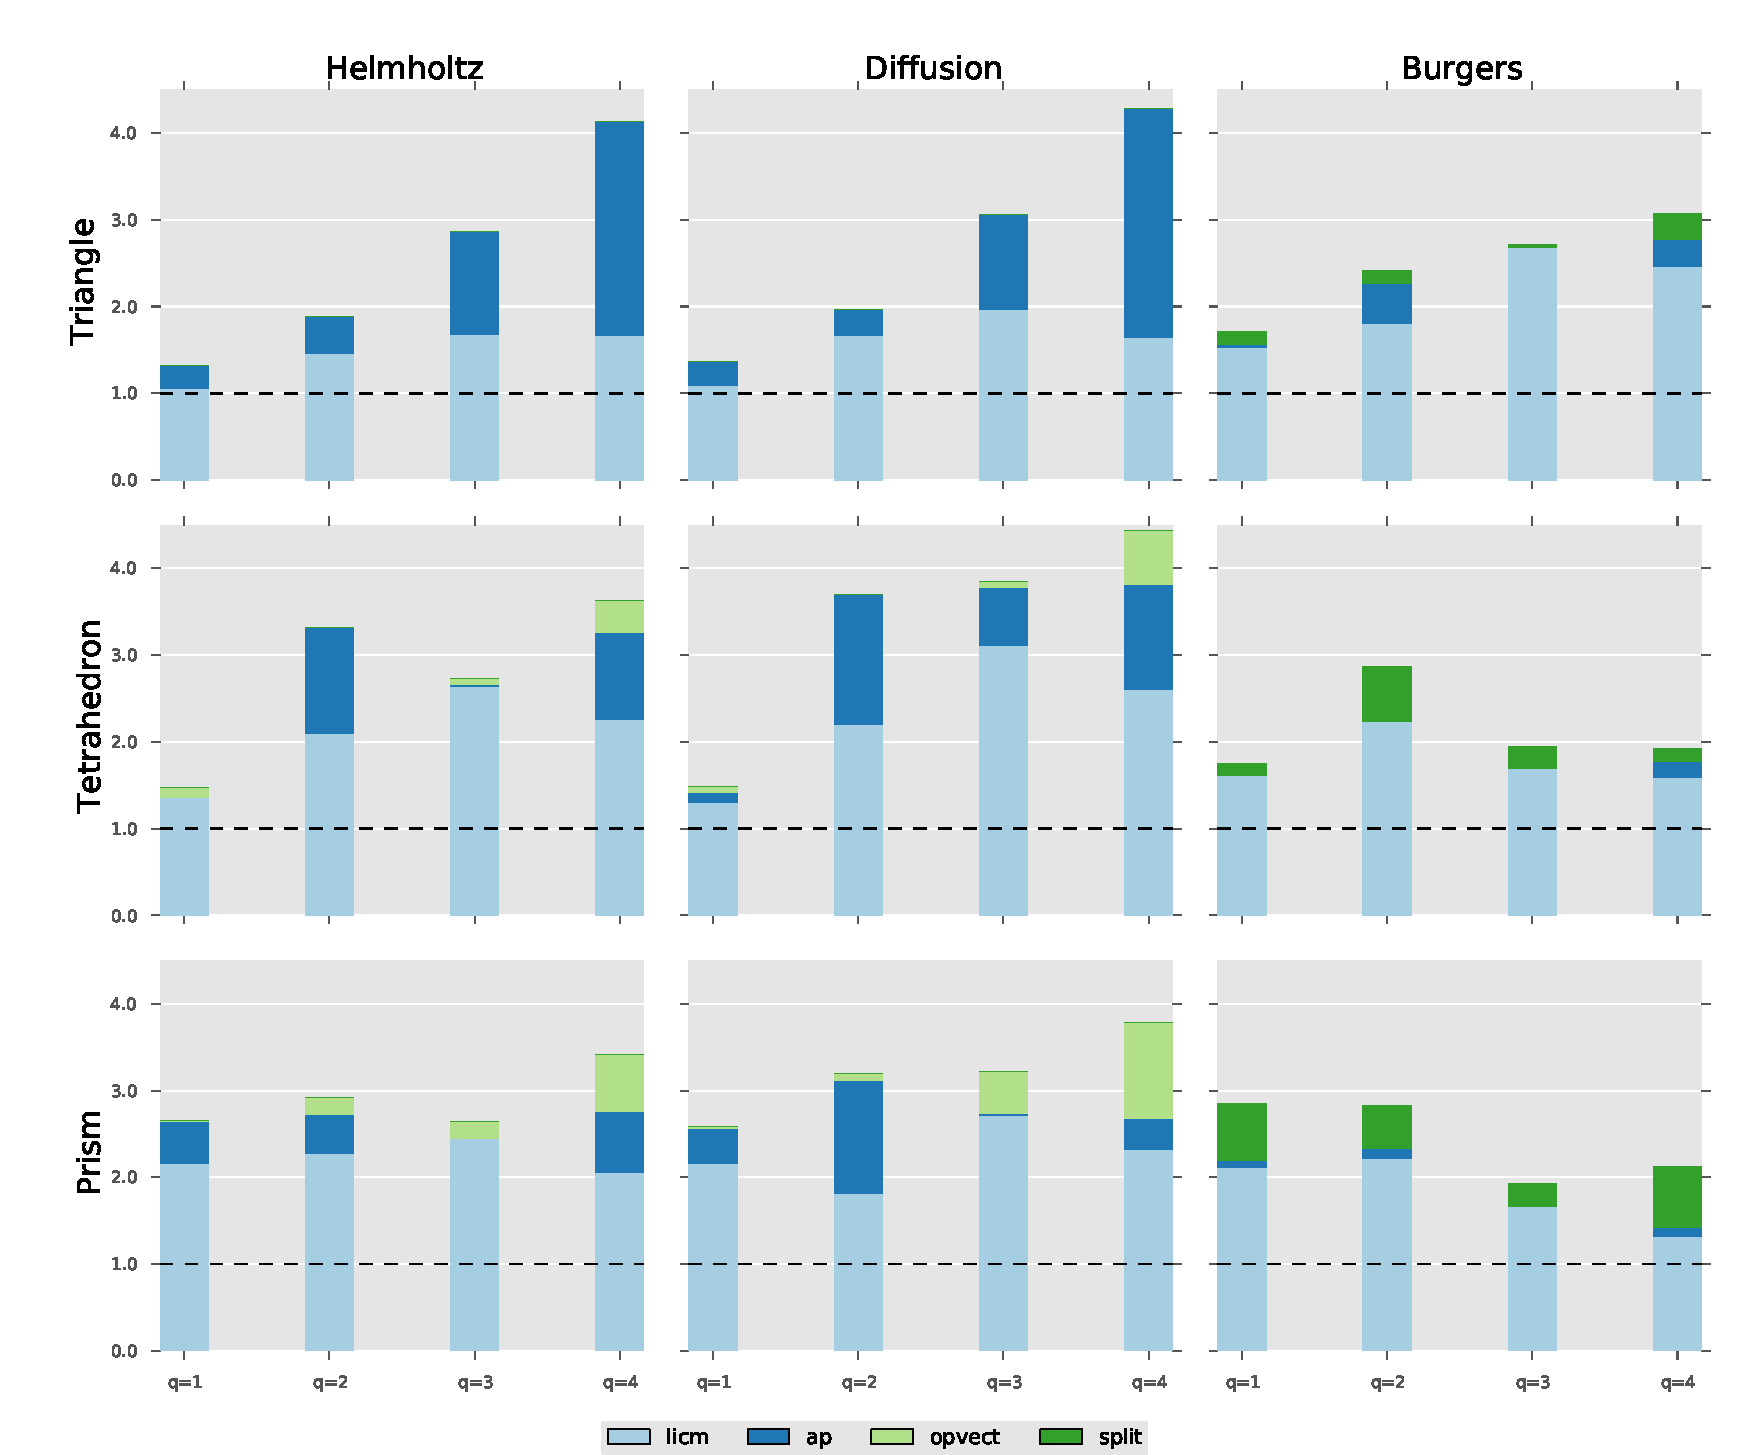
\includegraphics[scale=0.45]{coffee/perf-results/individual/graph}}
\caption{Performance improvement due to generalized loop-invariant code motion (\emph{licm}), data alignment and padding (\emph{ap}), outer-product vectorization (\emph{op-vect}), and expression splitting (\emph{split}) over the original non-optimized code. In each plot, the horizontal axis reports speed ups, whereas the polynomial order $q$ of the method varies along the vertical axis.}
\label{fig:coffee-individual-res}
\end{figure}

The speed ups due to applying optimizations over the original local assembly code are shown in Figure~\ref{fig:coffee-individual-res}. The figure itself can be read as a ``plot of plots'': the various element shapes are reported on the horizontal axis, whereas each equation corresponds to one point along the vertical axis. This allows to deduct the behaviour of transformations when varying the parameters of our study in an unified way. In the next sections, we refer to this figure and elaborate on the impact of individual transformations. We shorten generalized loop-invariant code motion as \emph{licm}; padding and data alignment as \emph{ap}; outer-product vectorization as \emph{op-vect}; expression splitting as \emph{split}.

\subsection{Impact of Transformations}
\subsubsection{Impact of Generalized Loop-invariant Code Motion}
\label{sec:perf-eval-licm}

In general, the speedups achieved by \emph{licm} are notable. The main reasons were anticipated in Section~\ref{sec:coffee-licm}: in the original code, 1) sub-expressions invariant to outer loops are not automatically hoisted, while 2) sub-expressions invariant to the innermost loop are hoisted, but their execution is not auto-vectorized. These observations come from inspection of assembly code generated by the compiler.

The gain tends to grow with the computational cost of the kernels: bigger loop nests (i.e., larger element shapes and polynomial orders) usually benefit from the reduction in redundant computation, even though extra memory for the temporary arrays is required. Some discrepancies to this trend are due to a less effective auto-vectorization. For instance, on the Sandy Bridge, the improvement at $q=3$ is larger than that at $q=4$ because, in the latter case, the size of the innermost loop is not a multiple of the vector length, and a remainder scalar loop is introduced at compile time. Since the loop nest is small, the cost of executing the extra scalar iterations can have a significant impact.

\subsubsection{Impact of Padding and Data Alignment}
\label{sec:perf-eval-padding}

Padding, which avoids the introduction of a remainder loop as described in Section~\ref{sec:coffee-padding}, as well as data alignment, enhance the quality of auto-vectorization. Occasionally the impact of \emph{ap} is marginal. These may be due to two reasons: (i) the non-padded element matrix size is already a multiple of the vector length; (ii) the number of aligned temporaries introduced by \emph{licm} is so large to induce cache associativity conflicts (e.g. Burgers equation).

\subsubsection{Impact of Vector-register Tiling}
\label{sec:perf-eval-opvect}

In this section, we evaluate the impact of vector-register tiling. \emph{op-vect} requires the unroll-and-jam factor to be explicitly set. Here, we report the best speed-up obtained after all feasible unroll-and-jam factors were tried. 

The rationale behind these results is that the effect of \emph{op-vect} is significant in problems in which the assembly loop nest is relatively big. When the loops are short, since the number of arrays accessed at every loop iteration is rather small (between 4 and 8 temporaries, plus the element matrix itself), there is no need for
vector-register tiling; extensive unrolling is sufficient to improve register re-use and, therefore, to maximize the performance. However, as the iteration space becomes larger, \emph{op-vect} leads to improvements up to 1.4$\times$ (Diffusion, prismatic mesh, $q=4$ - increasing the overall speed up from 2.69$\times$ to 3.87$\times$).

Using the Intel Architecture Code Analyzer tool~\cite{IACA}, we confirmed that speed ups are a consequence of increased register re-use. In Helmholtz $q=4$, for example, the tool showed that when using \emph{op-vect} the number of clock cycles to execute one iteration of the \texttt{j} loop decreases by roughly 17$\%$, and that this is a result of the relieved pressure on both of the data (cache) ports available in the core.

The performance of individual kernels in terms of floating-point operations per second was also measured. The theoretical peak on a single core, with the Intel Turbo Boost technology activated, is 30.4 GFlop/s. In the case of Diffusion using a prismatic mesh and $q=4$, we achieved a maximum of 21.9 GFlop/s with \emph{op-vect} enabled, whereas 16.4 GFlop/s was obtained when only \emph{licm-ap} is used. This result is in line with the expectations: analysis of assembly code showed that, in the \texttt{jk} loop nest, which in this problem represents the bulk of the computation, 73$\%$ of instructions are actually floating-point operations.

Application of \emph{op-vect} to the Burgers problem induces significant slowdowns due to the large number of temporary arrays that need to be tiled, which exceeds the available logical registers on the underlying architecture. Expression splitting can be used in combination with \emph{op-vect} to alleviate this issue; this is discussed in the next section.

%for which efficient register allocation can be already guaranteed

\subsubsection{Impact of Expression Splitting}
\label{sec:perf-results-split} 
Expression splitting relieves the register pressure when the element matrix evaluation needs to read from a large number of basis function arrays. As detailed in Section~\ref{sec:coffee-split}, the price to pay for this optimazion is an increased number of accesses to the element matrix and, potentially, redundant computation. 

For the Helmholtz and Diffusion kernels, in which only between 4 and 8 temporaries are read at every loop iteration, \texttt{split} tends to slow down the computation, because of the aforementioned drawbacks. Slow downs up to 1.4$\times$ were observed. 

In the Burgers kernels, between 12 and 24 temporaries are accessed at every loop iteration, so \emph{split} plays a key role since the number of available logical registers on the Sandy Bridge architecture is only 16. In almost all cases, a split factor of 1, meaning that the original expression was divided into two parts, ensured close-to-peak perforance. The transformation negligibly affected register locality, so speed ups up to 1.5$\times$ were observed. For instance, when $q=4$ and a prismatic mesh is employed, the overall performance improvement increases from 1.44$\times$ to 2.11$\times$. 

The performance of the Burgers kernel on a prismatic mesh was 20.0 GFlop/s from $q=1$ to $q=3$, while it was 21.3 GFlop/s in the case of $q=4$. These values are notably close to the peak performance of 30.4 GFlop/s. Disabling \emph{split} makes the performance drop to 17.0 GFlop/s for $q=1, 2$, 18.2 GFlop/s for $q=3$,
and 14.3 GFlop/s for $q=4$. These values are in line with the speedups shown in Figure~\ref{fig:coffee-individual-res}.

The \emph{split} transformation was also tried in combination with \emph{op-vect} (\emph{split-op-vect}). Despite improvements up to 1.22$\times$, \emph{split-op-vect} never outperforms \emph{split}. This is motivated by two factors: for small split factors, such as 1 and 2, the data space to be tiled is still too big, and register spilling affects run-time; for higher ones, sub-expressions become so small that, as explained in Section~\ref{sec:perf-eval-opvect}, extensive unrolling already allows to achieve a certain degree of register re-use.

\subsection*{Results on Other Architectures}
To avoid impairing the readability of the section, which already contains a vast amount of information, we are not reporting performance results on the Intel Xeon Phi  architecture (each core running at 1.05Ghz in native mode, 32KB L1 cache and 512KB L2 cache). With respect to the Sandy Bridge, this architecture has a different number of logical registers and SIMD lanes (16 256-bit registers in the Sandy Bridge, and 32 512-bit registers in the Xeon Phi), which can impact the optimization strategy. The interested reader is invited to refer to the published paper~\citep{Luporini-coffee}.


\section{Experience with General-purpose Compiler Optimizations}
\label{sec:coffee-genpurp-opts}

\subsection{Loop Interchange}
\label{sec:coffee-genpurp-opts-interchange}
All loops are interchangeable, provided that temporaries are introduced if the nest is not perfect. For the employed storage layout, the loop permutations \texttt{ijk} and \texttt{ikj} are likely to maximize performance. Conceptually, this is motivated by the fact that if the \texttt{i} loop were in an inner position, then a significantly higher number of load instructions would be required at every iteration. We tested this hypothesis in manually crafted kernels. We found that the performance loss is greater than the gain due to the possibility of accumulating increments in a register, rather than memory, along the \texttt{i} loop. The choice between \texttt{ijk} and \texttt{ikj} depends on the number of load instructions that can be hoisted out of the innermost dimension. As discussed in the next sections, a good heuristics it to choose as outermost the loop along which the number of invariant loads is smaller so that more registers remain available to carry out the computation of the local element matrix.

\subsection{Loop Unroll}
Loop unroll (or unroll-and-jam of outer loops) is fundamental to the exposure of instruction-level parallelism, and tuning unroll factors is particularly important.

We first observe that manual full (or extensive) unrolling is unlikely to be effective for two reasons. Firstly, the \texttt{ijk} loop nest would need to be small enough such that the unrolled instructions do not exceed the instruction cache, which is rarely the case: it is true that in a local assembly kernel the minimum size of the \texttt{ijk} loop nest is 3$\times$3$\times$3 (triangular mesh and polynomial order 1), but this increases rapidly with the polynomial order of the method and the discretization employed (e.g. tetrahedral meshes imply larger loop nests than triangular ones), so sizes greater than 10$\times$10$\times$10, for which extensive unrolling would already be harmful, are in practice very common. Secondly, manual unrolling is dangerous because it may compromise compiler auto-vectorization by either removing loops (most compilers search for vectorizable loops) or losing spatial locality within a vector register.

By comparison with implementations characterized by manually-unrolled loops, we noticed that recent versions of compilers like GNU's and Intel's estimate close-to-optimal unroll factors when the loops are affine and their bounds are relatively small and known at compile-time, which is the case of our kernels. Unless an auto-tuning system is used (this option is discussed in Section~\ref{sec:coffee-autotune}) our choice is to leave the backend compiler in charge of applying loop unroll. 

%TODO: maybe we can clarify that unroll-and-jam for opvect corresponds to changing the tile size...



\section{Related Work}
\label{sec:coffee-related-work}
The finite element method is extensively used to approximate solutions of PDEs. Well-known frameworks and applications include nek5000~\citep{nek5000-web-page}, the FEniCS project~\citep{Fenics}, Fluidity~\citep{fluidity_manual_v4}, and of course Firedrake. Numerical integration based on quadrature, as in Firedrake, is usually employed to implement the local assembly phase. The recent introduction of domain specific languages (DSLs) to decouple the finite element specification from its underlying implementation facilitated, however, the development of novel approaches. Methods based on tensor contraction~\citep{FFC-Compiler} and symbolic manipulation~\citep{francis} have been implemented. Nevertheless, it has been demonstrated that quadrature-based integration remains the most efficient choice for a wide class of problems~\citep{quadrature-olegaard}, which motivates our work in COFFEE.

Optimization of quadrature-based local assembly for CPU architectures has been addressed in FEniCS~\cite{quadrature-olegaard}. The comparison between COFFEE and this work has been presented in Section~\ref{sec:coffee-allforms-perf}. In~\citep{Markall20101815}, and more recently in~\citep{petsc-integration-gpu}, the same problem has been studied for GPU architectures. In~\citep{assembly-opencl}, variants of the standard numerical integration algorithm have been specialized and evaluated for the PowerXCell processor, but an exhaustive study from the compiler viewpoint - like ours - is missing, and none of the optimizations presented in this chapter are mentioned. Among these efforts, to the best of our knowledge, COFFEE is the first work targeting low-level optimizations through a real compiler approach.

The code transformations presented are inspired by standard compilers optimizations and exploit domain properties. Our loop-invariant code motion technique individuates invariant sub-expressions and redundant computation by analyzing all loops in an iteration space, which is a generalization of the algorithms often implemented by general-purpose compilers. Expression splitting is an abstract variant of loop fission based on properties of arithmetic operators. The outer-product vectorization is an implementation of tiling at the level of vector registers; tiling, or ``loop blocking'', is commonly used to improve data locality (especially for caches). Padding has been used to achieve data alignment and to improve the effectiveness of vectorization. A standard reference for the compilation techniques re-adapted in this work is~\citep{dragonbook}.

Our compiler-based optimization approach is made possible by the top-level DSL, which enables automated code generation. DSLs have been proven successful in auto-generating optimized code for other domains: Spiral~\citep{Pueschel:05} for digital signal processing numerical algorithms, ~\citep{Spampinato:14} for dense linear algebra, or Pochoir~\citep{pochoir} and SDSL~\citep{stencil-compiler} for image processing and finite difference stencils. Similarly, PyOP2 is used by Firedrake to express iteration over unstructured meshes in scientific codes. COFFEE improves automated code generation in Firedrake.

Many code generators, like those based on the Polyhedral model~\citep{pluto} and those driven by domain-knowledge~\citep{modeldriven}, make use of cost models. The alternative of using auto-tuning to select the best implementation for a given problem on a certain platform has been adopted by nek5000~\citep{nek5000} for small matrix-matrix multiplies, the ATLAS library~\citep{ATLAS}, and FFTW~\citep{FFTW} for fast fourier transforms. In both cases, pruning the implementation space is fundamental to mitigate complexity and overhead. Likewise, COFFEE uses heuristics and a model-driven auto-tuning system (Section~\ref{sec:coffee-autotune}) to steer the optimization process.


\section{Generality of the Approach and Applicability to Other Domains}
\label{sec:generality}
We have demonstrated that our cross-loop optimizations for arithmetic intensity are effective in the context of automated code generation for finite element local assembly. In this section, we discuss their applicability in other computational domains and, in general, their integrability within a general-purpose compiler.

COFFEE was developed as a separate, self-contained software module, with clear input/output interfaces, rather then incorporating it within PyOP2. This choice was motivated by two critical aspects that characterize the generality of our research:

\paragraph{Separation of concerns} We believe that in domain-specific frameworks there must be a clear, logical separation of roles reflecting the various levels of abstraction, where domain specialists are completely separated from performance optimization. In Firedrake, for instance, COFFEE decouples the mathematical specification of a finite element method, captured by the Unified Form Language and the FEniCS Form Compiler, from code optimization. This is of fundamental importance to maximize productivity by allowing scientists to focus only on their area of expertise. Practically speaking, from the perspective of the domain-specific language and compiler designers, our optimization strategy represents an incentive to produce extremely simple representations of the code (e.g. fully-inlined mathematical expressions in the form of an abstract syntax tree, in the case of Firedrake) so as to make the architecture-aware code optimizer completely responsible for choosing and applying the most suitable set of transformations.

\paragraph{Generalizability to other domains} There are neither conceptual nor technical reasons which prevent our compiler from being used in applications other than Firedrake. For example, integration with the popular FEniCS framework, the pioneer of automated code generation for finite element local assembly, would be relatively easy to achieve. It is more challenging to assess the generality of the optimization strategy: the extent to which COFFEE and its transformations are transferable to other computational domains, perhaps other DSLs, and to what extent this would be helpful for improving full application performance. To answer these questions, we first need to go back to the origins of our compiler. The starting point of our work was the mathematical formulation of a local assembly operation, expressible as follows

\begin{equation}
\label{eq:assembly-model}
\scriptsize
\forall_{i, j} ~~~ A_{ij}^K = \sum_{q=1}^{n_1} \sum_{k=1}^{n_2} \alpha_{k, q}(a', b', c', ...) \beta_{q, i, j}(a, b, c, d, ...) \gamma_{q}(w_K, z_K)
\end{equation}

The expression represents the numerical evaluation of an integral at $n_1$ points in the mesh element $K$ computing the local element matrix $A$. Functions $\alpha$, $\beta$ and $\gamma$ are problem-specific and can be intricately complex, involving for example the evaluation of derivatives. We can however abstract from the inherent structure of $\alpha$, $\beta$ and $\gamma$ to highlight a number of aspects

\begin{itemize}
\item \textbf{Optimizing mathematical expressions.} Expression manipulation (e.g. simplification, decomposition into sub-expressions) opens multiple semantically equivalent code generation opportunities, characterized by different trade-offs in parallelism, redundant computation, and data locality. The basic idea is to exploit properties of arithmetic operators, such as associativity and commutativity, to re-schedule the computation suitably for the underlying architecture. Loop-invariant code motion and expression splitting follow this principle, so they can be re-adapted or extended to any domains involving numerical evaluation of complex mathematical expressions (e.g. electronic structure calculations in physics and quantum chemistry relying on tensor contractions~\cite{TCE}). In this context, we highlight three notable points.
\begin{enumerate}
\item In Equation~\eqref{eq:assembly-model}, the summations correspond to reduction loops, whereas loops over indices $i$ and $j$ are fully parallel. Throughout the paper we assumed that a kernel will be executed by a single thread, which is likely to be the best strategy for standard multi-core CPUs. On the other hand, we note that for certain architectures (for example GPUs) this could be prohibitive due to memory requirements. Intra-kernel parallelization is one possible solution: a domain-specific compiler such as COFFEE could map mathematical quantifiers and operators to different parallelization schemes and generate distinct variants of multi-threaded kernel code. Based on our experience, we believe this is the right approach to achieve performance portability.
\item The various sub-expressions in $\beta$ only depend on (i.e. iterate along) a subset of the enclosing loops. In addition, some of these sub-expressions might reduce to the same values as iterating along certain iteration spaces. This code structure motivated the generalized loop-invariant code motion technique. The intuition is that whenever sub-expressions invariant with respect to different sets of affine loops can be identified, the question of whether, where and how to hoist them, while minimizing redundant computation, arises. Pre-computation of invariant terms also increases memory requirements due to the need for temporary arrays, so it is possible that for certain architectures the transformation could actually cause slowdowns (e.g. whenever the available per-core memory is small).
\item Associative arithmetic operators are the prerequisite for expression splitting. In essence, this transformation concerns resource-aware execution. In the context of COFFEE, expression splitting has been successfully applied to improve register pressure. However, the underlying idea of re-scheduling (re-associating) operations to optimize for some generic parameters is far more general. It could be used, for example, as a starting point to perform kernel fission; that is, splitting a kernel into multiple parts, each part characterized by less stringent memory requirements (a variant of this idea for non-affine loops in unstructured mesh applications has been adopted in~\citep{op2-lcpc}). In Equation~\eqref{eq:assembly-model}, for instance, not only can any of the functions $\alpha$, $\beta$ and $\gamma$ be split (assuming they include associative operators), but $\alpha$ could be completely extracted and evaluated in a separate kernel. This would reduce the working set size of each of the kernel functions, an option which is particularly attractive for many-core architectures in which the available per-core memory is much smaller than that in traditional CPUs.
\end{enumerate}
\item \textbf{Code generation and applicability of the transformations.} All array sizes and loop bounds, for example $n1$ and $n2$ in Equation~\ref{eq:assembly-model}, are known at code generation time. This means that ``good'' code can be generated. For example, loop bounds can be made explicit, arrays can be statically initialized, and pointer aliasing is easily avoidable. Further, all of these factors contribute to the applicability and the effectiveness of some of our code transformations. For instance, knowing loop bounds allows both generation of correct code when applying vector-register tiling and discovery of redundant computation  opportunities. Padding and data alignment are special cases, since they could be performed at run-time if some values were not known at code generation time. Theoretically, they could also be automated by a general-purpose compiler through profile-guided optimization, provided that some sort of data-flow analysis is performed to ensure that the extra loop iterations over the padded region do not affect the numerical results. 
\item \textbf{Multi-loop vectorization.} Compiler auto-vectorization has become increasingly effective in a variety of codes. However, to the best of our knowledge, multi-loop vectorization involving the loading and storing of data along a subset of the loops characterizing the iteration space (rather than just along the innermost loop), is not supported by available general-purpose and polyhedral compilers. The outer-product vectorization technique presented in this paper shows that two-loop vectorization can outperform standard auto-vectorization. In addition, we expect the performance gain to scale with the number of vectorized loops and the vector length (as demonstrated in  the Xeon Phi experiments). Although the automation of multi-loop vectorization in a general-purpose compiler is far from straightforward, especially if stencils are present, we believe that this could be more easily achieved in specific domains. The intuition is to map the memory access pattern onto vector registers, and then to exploit in-register shuffling to minimize the traffic between memory and processor. By demonstrating the effectiveness of multi-loop vectorization in a real scenario, our research represents an incentive for studying this technique in a broader and systematic way.
\end{itemize}

\section{Conclusion}
\label{sec:coffee-conclusion}
In this chapter, we have presented the study and systematic performance evaluation of a class of composable cross-loop optimizations for improving arithmetic intensity in finite element local assembly kernels, and their integration in a novel compiler, COFFEE. In the context of automated code generation for finite element local assembly, COFFEE is the first compiler capable of introducing low-level optimizations to maximize instruction-level parallelism, register locality and SIMD vectorization. Assembly kernels have particular characteristics. Their iteration space is usually very small, with the size depending on aspects like the degree of accuracy one wants to reach (polynomial order of the method) and the mesh discretization employed. The data space, in terms of number of arrays and scalars required to evaluate the element matrix, grows proportionally with the complexity of the finite element problem. COFFEE has been developed taking into account all of these degrees of freedom, based on the idea that reducing the problem of local assembly optimization to a fixed sequence of transformations is far too superficial if close-to-peak performance needs to be reached. The various optimizations overcome limitations of current vendor and research compilers. The exploitation of domain knowledge allows some of them to be particularly effective, as demonstrated by our experiments on a state-of-the-art Intel platform. COFFEE supports all of the problems expressible in Firedrake, and is integrated with this framework, which demonstrate the maturity of the research performed. The generality and the applicability of the proposed code transformations to other domains has also been discussed.
